%%%%%%%%%%%%%%%%%%%%%%%%%%%%%%%%%%%%%%%%%
% Thin Sectioned Essay
% LaTeX Template
% Version 1.0 (3/8/13)
%
% This template has been downloaded from:
% http://www.LaTeXTemplates.com
%
% Original Author:
% Nicolas Diaz (nsdiaz@uc.cl) with extensive modifications by:
% Vel (vel@latextemplates.com)
%
% License:
% CC BY-NC-SA 3.0 (http://creativecommons.org/licenses/by-nc-sa/3.0/)
%
%%%%%%%%%%%%%%%%%%%%%%%%%%%%%%%%%%%%%%%%%

%----------------------------------------------------------------------------------------
%	PACKAGES AND OTHER DOCUMENT CONFIGURATIONS
%----------------------------------------------------------------------------------------

\documentclass[a4paper, 11pt]{article} % Font size (can be 10pt, 11pt or 12pt) and paper size (remove a4paper for US letter paper)

\usepackage[protrusion=true,expansion=true]{microtype} % Better typography
\usepackage{graphicx} % Required for including pictures
\usepackage{wrapfig} % Allows in-line images

\usepackage{mathpazo} % Use the Palatino font
\usepackage[T1]{fontenc} % Required for accented characters
\linespread{1.05} % Change line spacing here, Palatino benefits from a slight increase by default

\makeatletter
\renewcommand\@biblabel[1]{\textbf{#1.}} % Change the square brackets for each bibliography item from '[1]' to '1.'
\renewcommand{\@listI}{\itemsep=0pt} % Reduce the space between items in the itemize and enumerate environments and the bibliography

\renewcommand{\maketitle}{ % Customize the title - do not edit title and author name here, see the TITLE block below
\begin{flushright} % Right align
{\LARGE\@title} % Increase the font size of the title

\vspace{50pt} % Some vertical space between the title and author name

{\large\@author} % Author name
\\\@date % Date

\vspace{40pt} % Some vertical space between the author block and abstract
\end{flushright}
}

%----------------------------------------------------------------------------------------
%	TITLE
%----------------------------------------------------------------------------------------

\title{\textbf{The Stallion}\\ % Title
Group 9 Project Report\\DD2425} % Subtitle

\author{\textsc{
Tobias Andersson\\
Max Losch\\
Diego Martinez Marrodan\\
Tiago Sebastiao\\
Lan Wang} % Author
\\{\textit{Royal Institute of Technology}}
} % Institution

\date{\today} % Date

%----------------------------------------------------------------------------------------

\begin{document}

\maketitle % Print the title section

%----------------------------------------------------------------------------------------
%	ABSTRACT
%----------------------------------------------------------------------------------------

%\renewcommand{\abstractname}{Summary} % Uncomment to change the name of the abstract to something else

\begin{abstract}
Morbi tempor congue porta. Proin semper, leo vitae faucibus dictum, metus mauris lacinia lorem, ac congue leo felis eu turpis. Sed nec nunc pellentesque, gravida eros at, porttitor ipsum. Praesent consequat urna a lacus lobortis ultrices eget ac metus. In tempus hendrerit rhoncus. Mauris dignissim turpis id sollicitudin lacinia. Praesent libero tellus, fringilla nec ullamcorper at, ultrices id nulla. Phasellus placerat a tellus a malesuada.
\end{abstract}

\vspace{30pt} % Some vertical space between the abstract and first section

%----------------------------------------------------------------------------------------
%	ESSAY BODY
%----------------------------------------------------------------------------------------

\section{Vision}

Although the main intent of the vision was to detect the given set of objects (see figure \ref{fig:object_set},
it was later on also used to exploit wall and ground information for mapping and localization functionality.

\begin{figure}
\begin{center}
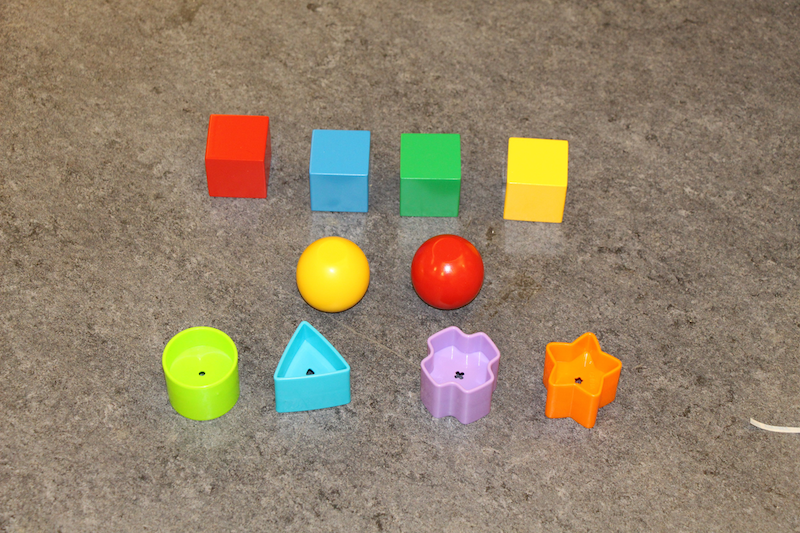
\includegraphics[width=0.38\textwidth]{figures/object_dataset}
\end{center}
\caption{Object data set}
\label{fig:object_set}
\end{figure}

The vision part of the project can be divided in 3 different parts.
They are object detection, shape recognition and color recognition.
While both shape and color recognition both rely on the accuracy and overall results of the object detection algorithm, they are totally independent. 
The final result of the whole object recognition part of the project is done after having reliable data form each of the components, color and shape.
In this part we chose to implement everything upon the Point Cloud Library. 
This choice is based on the added functionality of actually being able to represent the objects and walls and ground by points in 3D and not in a 2D picture. 
And such having more information about the object structure and additionally being less dependent on illumination changes.
Of course it is possible to convert between these two representations, but the PCL library has already a lot of useful functions that were able to decrease the amount of data manipulation.

\subsection{Object Detection}

The main idea is that we know that the objects are at ground level.
If we can detect the ground, we can then set some boundaries on the presence of the object above it, hence increasing the chances of detecting an object.
So the first part was find the walls and ground. Here, RANSAC was used. This algorithm exploits the fact that we are trying to find a special kind of order (model) among our data.
In our case, our data is the point cloud at a given time and the model are planes. 
By trying to fit planes in the point cloud, the algorithm is able to distinguish between inliers, points in some specific plane, and outliers, like noise or indeed the objects we are trying to find.
Now that we have the ground plane, we define a region of interest of about 5 cm high above it, where, if we can detect enough points, we will group them and afterwards classify them.
Note that it is possible to have 2 objects that satisfy the ground distance criteria and hence the conditions for an interesting group of points to exist is constrained by its size.
When this algorithm ends, we know one of two things:
\begin{enumerate}
\item there is no object in the frame
\item there is at least one region of interest
\end{enumerate}

\begin{figure}
\begin{center}
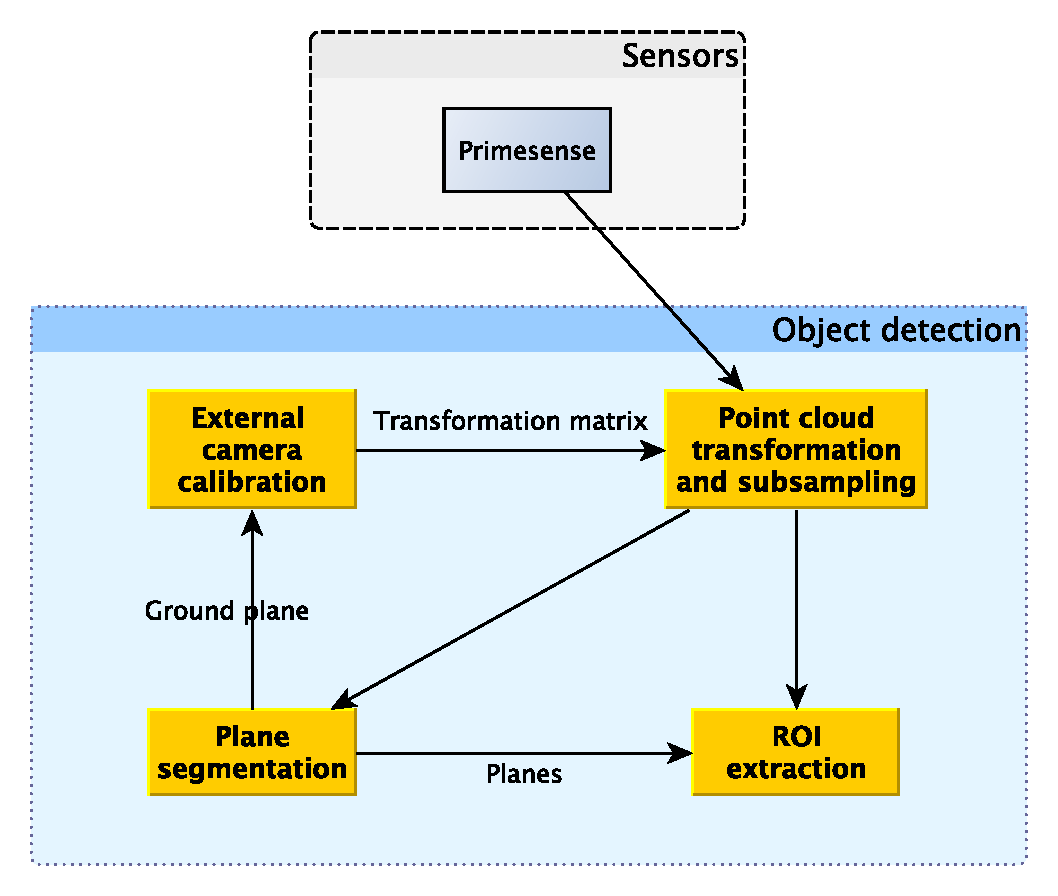
\includegraphics[width=0.45\textwidth]{figures/arch_vision_obj_det.pdf}
\end{center}
\caption{Object detection - Process flow}
\label{fig:vision:obj_det}
\end{figure}
 
\subsection{Object recognition} 
 
\subsection{Shape Recognition}

In this section we explain our logic behind the shape recognition algorithm.
The general idea was again model fitting.
We know about 3 very specific models that we want to try, cube, cylinder and sphere, and we have two objects with no general model.
The PCL library has available the RANSAC algorithm to fit some predifined models, like planes, spheres and cylinders. 
And that is what we used. 
The sphere fitting and cylinder are straightforward since they work exactely like the plane fitting mentioned above, the only difference being that the model is no longer a plane.
Hence they work in similar way as the plane fitting.
The big difference is the cube.
To recognize a cube we do plane fitting too, but we impose some conditions of the planes.

\begin{enumerate}
\item if 3 planes are detected then it's a cube
\item there has to be a parallel plane relative to the ground
\item distance between the ground plane and the parallel plane described above must be reasonable
\item the furthest plane must be the parallel plane
\end{enumerate}

The constraints above limit the possibility of noise being misclassified, as well as other shapes being mischaracterized.
There was obviously some empirical testing in order to find the best parameters for the RANSAC model fitting, like: 

\begin{itemize}
\item MAX:: I know some of them but can't remember their function
\end{itemize}


\subsection{Color Recognition}

Extracting the color values from an image, or in our case from points, is not a hard task. 
However, to give meaning to those values is harder, since the color itself depends on a rather large number of factors like available light, its intensity, its color, among others.
This makes it hard to obtain a robust but consistent color recognition algorithm.
Our approach was very empirical. The analysis is made per color possible and not all at once, even though the algorithm is the same whatever the color.
We started by analising the HSV (hue, saturation, value) values we got from the regions of interest, mainly the hue, which is what defines the color. 
We then tried to find meaning in those values, mainly their average.
We concluded that for the most part, the overall average of hues of all the points in the region of interest would be enough to obtain a good estimate of the color. 
So we defined an area our each color mean value around which the color will be.
The bigger the margin, the more robust the algorithm would be.
However, because of the specific colors, the margin could not be too large, or the added robustness would not be reliable, as colors would start to mix.
Because different conditions may lead to very different results, we weighted two times the previous result based on specific situations, mainly, the percentage of points that have the color being tested relative to the total number of points, and the probability of being of the color being analysed, i.e., considering the point clouds don't usually have that many points, we give a higher weight to probabilities above a certain value.
Because the blob of interest may have points not only belonging to the object we want, but also from the ground or wall (if the object is very close to one), the number of points that have a color similar to orange, color of the ground, is also relevant in deciding the true color of the object, and hence helps in determining the weight of the probability of the color being analysed.
The end result is a somewhat robust algorithm and consistent as far as our testing went. 

\begin{figure}
\begin{center}
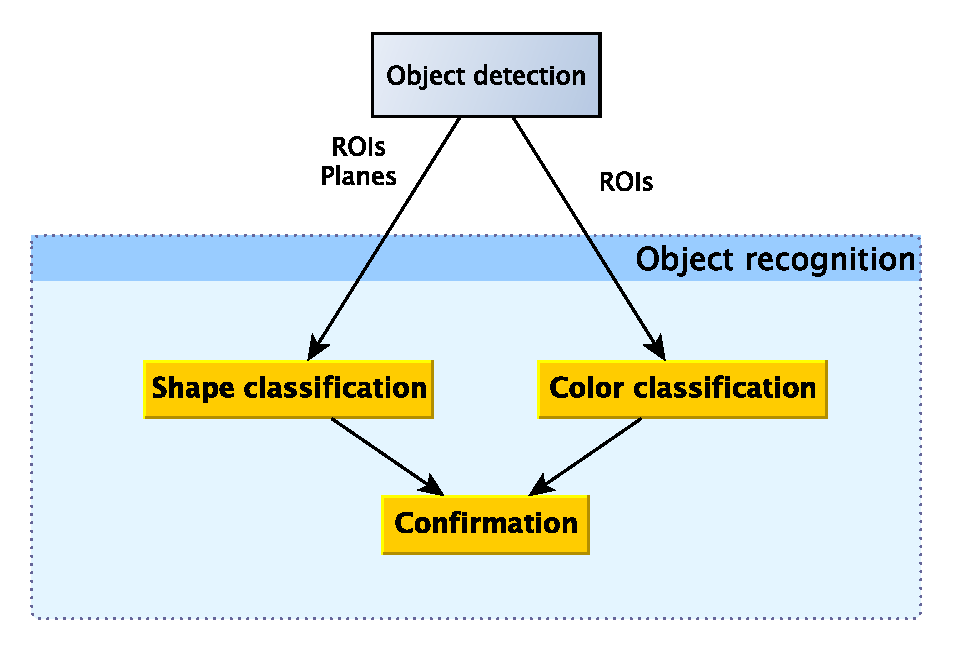
\includegraphics[width=0.45\textwidth]{figures/arch_vision_obj_rec.pdf}
\end{center}
\caption{Object recognition - Process flow}
\label{fig:vision:obj_rec}
\end{figure}
\input{sections/Localization}
\section{Controlling}

The main task of the project requires the robot to move with the highest possible speed.
On the other hand the robot should be able to move at a speed that induces as little drift as possible and reduces the risk of errors when hitting an obstacle.
And lastly, the vision would have to identify objects from further away, increasing the difficulty of implementation and recognition.
Thus, a balance in the velocities have to be found.\\

The implemented controllers consisted of a forward movement controller, a turn controller and a wall alignment controller.
By embedding them in an adapter pattern it was possible to render their usage very versatile (see figure \ref{fig:arch_controller}).
Every controller inherited hereby a controller base which defined an interface that updated the logic and returned a Twist
(A Twist is one of many ros pre-baked data structures that can be sent as a message. 
It stores a position and a rotation). 
The adapter combines all received Twists to one Twist, entrusting that no contradictions occur.
A top logic has to ensure that the right controllers are activated and deactivated.
This can be done by activating and deactivating each controller.
Controllers like the turn and the forward movement controller respond with a message as soon as they have stopped or finished their activity.\\

\begin{figure}[h]
\begin{center}
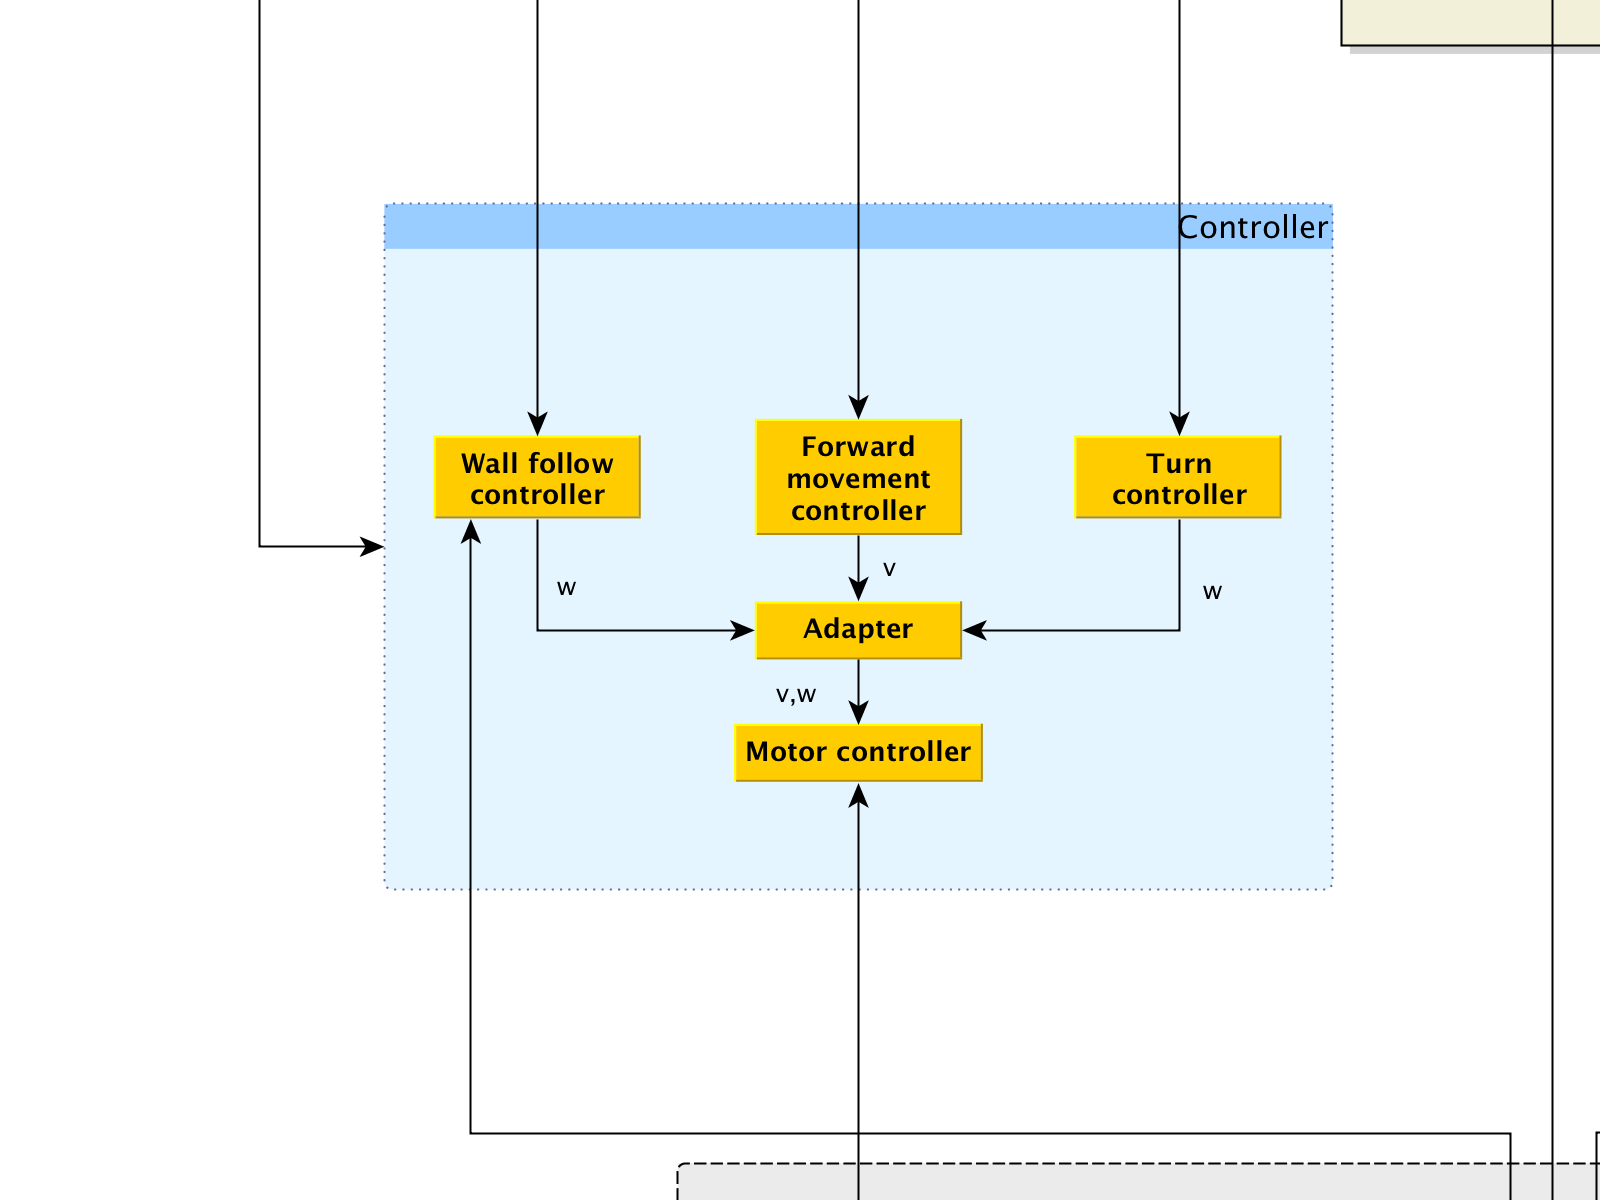
\includegraphics[width=0.6\textwidth]{figures/arch_controller.png}
\end{center}
\caption{Architecture of the controller package}
\label{fig:arch_controller}
\end{figure}

\subsection{Motor controller}

Due to internal motor difference, it is not sufficient to control the motors directly.
Otherwise the robot would move in an arch, one motor rotating slower than the other.
To compensate for that and to also be able to input linear and angular velocities, a PID controller was used. 
This enabled the robot to drive in a stable straight line.

The motors itself have a static resistance, that have to be overcome whenever the motors should transition from idling to rotating.
Overcoming these static resistance could be described by constants (for each motor one) $K_{power}$, that were added to the result of the PID results.
As soon as the static resistance has been overcome and the motor is rotating, the constant $K_{power}$ can be reduced to a value that sustains rotation: $K_{sustain}$.
This behavior results in a spiked motor control output as can be seen in figure \ref{fig:pwm_spiker}.
Although movement without spiking is possible due to the accumulating behavior of the PID controller too, it ensures responsive controlling and avoids the necessecity of increasing the gains which can easily result in overshoots.

\begin{figure}[h]
\begin{center}
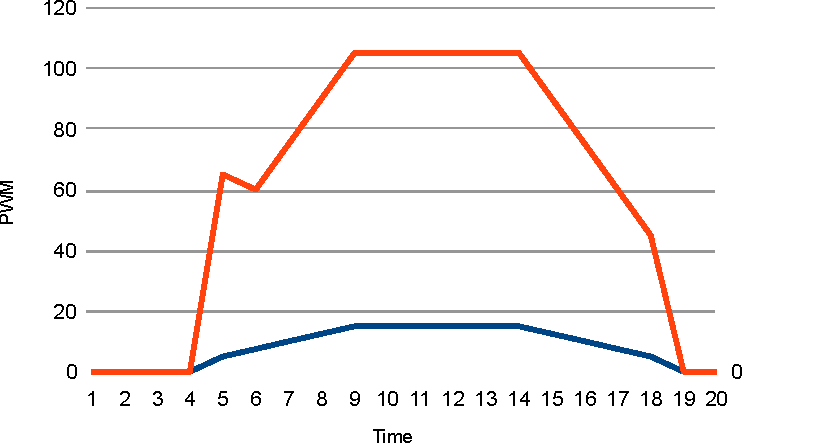
\includegraphics[width=0.6\textwidth]{figures/pwm_spike.pdf}
\end{center}
\caption{PWM Spiking for initial motor rotation attempt}
\label{fig:pwm_spiker}
\end{figure}

\subsection{Wall alignment}

The wall allignment controller (see figure \ref{fig:arch_controller}) uses the IR sensors to measure the distances from the robot to the walls, and works as follows: if both walls are close to the robot (distance < 0.4 m), then keep the robot aligned to the center between both walls.
Otherwise control only by the next closest wall, or if no wall is present, do not align.

\section*{Section Name}

Cras gravida, est vel interdum euismod, tortor mi lobortis mi, quis adipiscing elit lacus ut orci. Phasellus nec fringilla nisi, ut vestibulum neque. Aenean non risus eu nunc accumsan condimentum at sed ipsum.
\begin{wrapfigure}{l}{0.4\textwidth} % Inline image example
\begin{center}
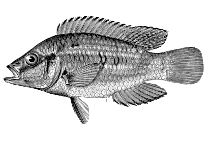
\includegraphics[width=0.38\textwidth]{fish.png}
\end{center}
\caption{Fish}
\end{wrapfigure}
Aliquam fringilla non diam sed varius. \cite{Smith:2012qr} Suspendisse tellus felis, hendrerit non bibendum ut, adipiscing vitae diam. Lorem ipsum dolor sit amet, consectetur adipiscing elit. Nulla lobortis purus eget nisl scelerisque, commodo rhoncus lacus porta. Vestibulum vitae turpis tincidunt, varius dolor in, dictum lectus. Aenean ac ornare augue, ac facilisis purus. Sed leo lorem, molestie sit amet fermentum id, suscipit ut sem. Vestibulum orci arcu, vehicula sed tortor id, ornare dapibus lorem. Praesent aliquet iaculis lacus nec fermentum. Morbi eleifend blandit dolor, pharetra hendrerit neque ornare vel. Nulla ornare, nisl eget imperdiet ornare, libero enim interdum mi, ut lobortis quam velit bibendum nibh.\cite{Smith:2013jd}

Morbi tempor congue porta. Proin semper, leo vitae faucibus dictum, metus mauris lacinia lorem, ac congue leo felis eu turpis. Sed nec nunc pellentesque, gravida eros at, porttitor ipsum. Praesent consequat urna a lacus lobortis ultrices eget ac metus. In tempus hendrerit rhoncus. Mauris dignissim turpis id sollicitudin lacinia. Praesent libero tellus, fringilla nec ullamcorper at, ultrices id nulla. Phasellus placerat a tellus a malesuada.

%------------------------------------------------

\section*{Conclusion}

Herpa derpa derp.

\begin{enumerate}
\item First numbered list item
\item Second numbered list item
\end{enumerate}

Donec luctus tincidunt mauris, non ultrices ligula aliquam id. Sed varius, magna a faucibus congue, arcu tellus pellentesque nisl, vel laoreet magna eros et magna. 

%----------------------------------------------------------------------------------------
%	BIBLIOGRAPHY
%----------------------------------------------------------------------------------------

\bibliographystyle{unsrt}

\bibliography{sample}

%----------------------------------------------------------------------------------------

\end{document}